\section{Modelli di Ciclo di Vita}

\begin{definition}[Processo Software]
    Con processo software si indica il percorso da seguire per sviluppare un prodotto o più nello specifico un software.
    Fanno parte del processo sia gli strumenti e le tecniche per lo sviluppo che i professionisti coinvolti.
\end{definition}

\subsection{Modelli Sequenziali}

\subsubsection{Build-and-Fix}

Il prodotto è sviluppato senza alcuna fase di progettazione preliminare, lo sviluppatore scrive il software
e poi lo modifica ogni volta che non soffisfa il committente.

\paragraph{\textcolor{red}{Contro}}

Diventa improponibile per progetti grandi e la manutenzione diventa difficile senza documentazione nè specifica.

\subsubsection{Modello a Cascata}

Questo modello è stato il primo a distingure il processo software in più fasi, evidenziando l'importanza della progettazione e dell'analisi.

Viene chiamato anche modello \emph{\textcolor{cyan}{document driven}} dato che ogni fase produce un documento, e per passare alla successiva
occorre aver approvato il documento della fase precedente.

\paragraph{\textcolor{red}{Contro}} Troppo pesante da seguire, inoltre non si può tornare indietro, e mancando
l'interazione con il cliente, se non è soddisfatto, và tutto ripetuto dall'inizio.

\subsubsection{Modello a V}

\begin{center}
    \begin{figure}[h]
            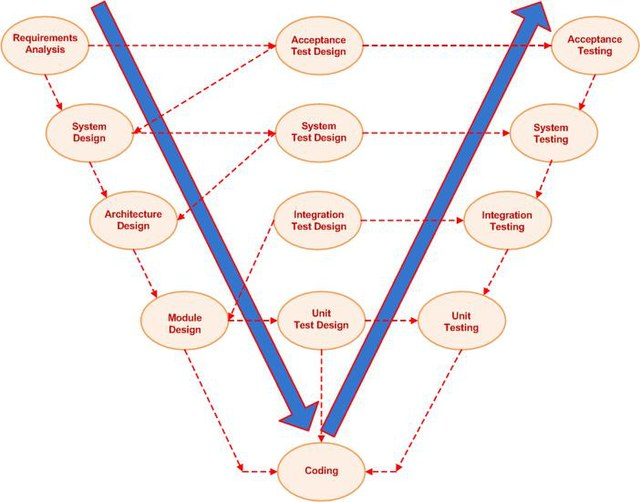
\includegraphics[scale=0.5]{img/V-model.JPG}
        \caption{Le frecce blu rappresentano il \emph{tempo}, mentre quelle tratteggiate le \emph{dipendenze}}
    \end{figure}
\end{center}

Questo modello evidenzia come sia possibile progettare i \textcolor{cyan}{test}
durante le fasi di sviluppo (quelle a sinistra, prima della fase di \emph{coding}). Mentre sulla destra
sono presenti i test veri e propri che devono verificare e convalidare l'attività in corrispondenza sulla sinistra.

\paragraph{\textcolor{ForestGreen}{Standard SQA}}
Questo modello è uno degli standard \emph{SQA} (Software Quality Assurance), usato
per descrivere le attività di test durante il processo di sviluppo.

\subsection{Modelli Iterativi}

\subsubsection{Rapid Prototyping}

L'obbiettivo è quello di costruire rapidamente un prototipo del software per permettere al committente di sperimentarlo.

Questo modello diventa utile quando i requisiti non sono chiari, quindi ogni prototipo aiuterà il cliente a descriverli meglio.

\begin{center}
    \begin{tikzpicture}[main/.style={rectangle, draw}]
        \node[main] (1) {Analisi Preliminare};
        \node[main] (2) [below right=1cm and 0.1cm of 1] {Analisi e Progettazione};
        \node[main] (3) [below right=1cm and 0.1cm of 2] {\begin{tabular}{c}Realizzazione del \\ prototipo (usa e getta)\end{tabular}};
        \draw[thick, ->] (1) -| (2);
        \draw[thick, ->] (2) -| (3);
        \draw[thick, ->] (3) -| (2);
    \end{tikzpicture}
\end{center}

\subsubsection{Modello Incrementale}

Il software viene costruito in modo iterativo, aggiungendo di volta in volta nuove funzionalità.

I requisiti e la progettazione vengono definiti inizialmente, per questo è possibile applicarlo solo in caso di requisiti stabili.

\paragraph{\textcolor{red}{Contro}}
Se non viene realizzata una buona progettazione, questo modello sfocia in un \emph{Build-and-Fix}.

\begin{center}
    \begin{tikzpicture}[main/.style={rectangle, draw}]
        \node[main] (1) {Analisi e Progettazione};
        \node[main] (2) [below right=0.5cm and -2cm of 1] {\begin{tabular}{c} Progettazione di dettaglio \\ (implemento una singola funzionalità) \end{tabular}};
        \node[main] (3) [below right=1cm and -1.5cm of 2] {\begin{tabular}{c} Realizzazione versione \\ incompleta \end{tabular}};
        \draw[thick, ->] (1) -| (2);
        \draw[thick, ->] (2) -| (3);
        \draw[thick, ->] (3) -| (2);
    \end{tikzpicture}
\end{center}

\newpage

\subsubsection{Modello a Spirale}

In questo caso ogni iterazione è formata da 4 fasi che corrispondono ai quadranti del piano:
\begin{enumerate}
    \item \emph{Quadrante in alto a sinistra}: definizione degli obiettivi e dei vincoli.
    \item \emph{Quadrante in alto a destra}: analisi e risoluzione dei rischi.
    \item \emph{Quadrante in basso a destra}: sviluppo e verifica del prossimo livello.
    \item \emph{Quadrante in basso a sinistra}: pianificazione della fase successiva.
\end{enumerate}

Questo modello viene anche chiamato \emph{\textcolor{cyan}{risk driven}} in quanto è incentrato principalmente sull'analisi
dei rischi. Inoltre si ispira profondamente al metodo iterazivo \emph{\textcolor{cyan}{plan-do-check-act cycle}} \footnote{\url{https://it.wikipedia.org/wiki/Ciclo_di_Deming}}

\begin{figure}[h]
    \begin{center}
        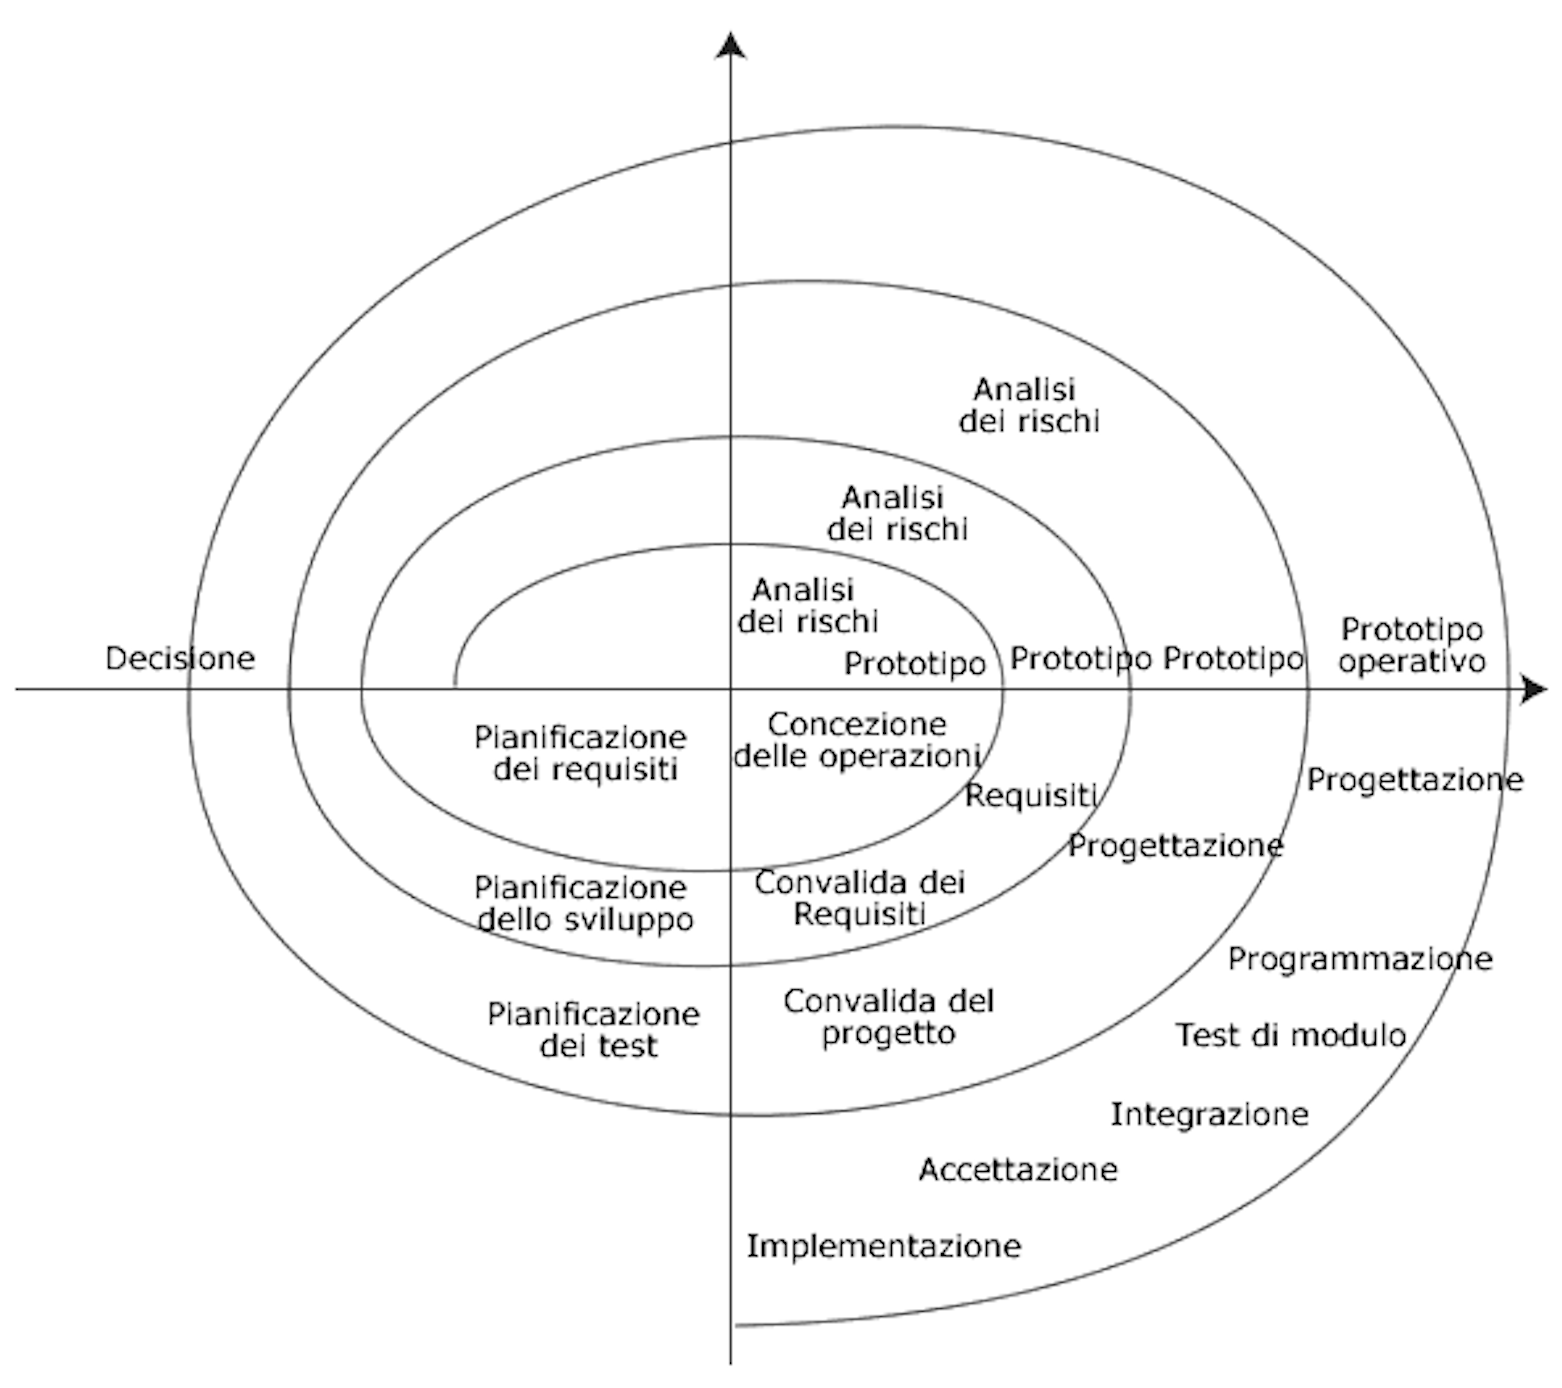
\includegraphics[scale=0.4]{img/modellospirale.png}
    \end{center}
\end{figure}

\subsection{Unified Process}

In questo modello vengono distinte quattro fasi chiamate \emph{\textcolor{cyan}{Inception}}, \emph{\textcolor{cyan}{Elaboration}}, \emph{\textcolor{cyan}{Construction}}
e \emph{\textcolor{cyan}{Transition}}. Ogni fase può presentare un numero variabile di iterazioni anche in base alla dimensione
del progetto.

Questo modello viene definito \textcolor{cyan}{iterativo incrementale}, \emph{incrementale} perchè
alla fine di ogni iterazione si ottiene un rilascio del sistema con funzionalità in più o migliorate
rispetto al rilascio precedente.

Inoltre viene data molta importanza all'architettura del sistema, infatti già dalle prime fasi ci si
concentra soprattutto sull'architettura anche se a livello molto superficiale, lasciando i dettagli alle fasi successive. In questo
modo è molto facile avere una visione generale del sistema che sarà facilmente modellabile sulla variazione dei requisiti. Per
questo, piuttosto che dai requisiti, ci si fà guidare principalmente dai \emph{casi d'uso} e dall'\emph{analisi dei rischi}.

\begin{figure}[h]
    \begin{center}
        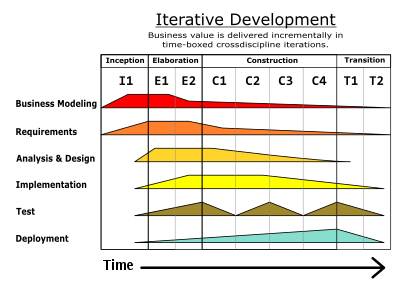
\includegraphics[scale=0.8]{img/unified_process.png}
    \end{center}
\end{figure}

\subsection{Processi Agili}